\chapter{Entropy lỗ đen, toàn ảnh và không gian de Sitter}

\lectureoverview{Chúng ta hoàn tất lập luận tương ứng đã bắt đầu ở bài giảng trước. Một dây kích thích mạnh có entropy tỉ lệ với khối lượng của nó, còn một lỗ đen Schwarzschild có entropy tỉ lệ với diện tích của nó. Hai công thức này được nối với nhau không phải bằng cách đồng nhất một lỗ đen tự hấp dẫn mạnh với một dây tự do, mà bằng cách biến thiên chậm hằng số ghép dây cho đến khi hai mô tả gặp nhau. Khi đó định luật diện tích dẫn một cách tự nhiên đến nguyên lý toàn ảnh, và phần cuối của bài giảng giới thiệu không gian giãn nở cùng hình học de Sitter, với chân trời của nó sẽ được khảo sát tiếp theo.}

\section{Trở lại bài toán đếm}

Có một điểm còn bỏ ngỏ trong phép đếm dây dài. Nếu một tổng chiều dài cố định được chia cho một số dây, các dây giống hệt nhau có cùng độ dài là không thể phân biệt được. Tuy vậy, vị trí của chúng trong hộp vẫn là một phần của trạng thái, và hộp được chọn có kích thước xấp xỉ vùng mà một dây dài đơn lẻ tương ứng chiếm giữ.

\begin{classroomqa}
\audiencequestion{Các dây ngắn có được phân biệt với nhau không, và vị trí của chúng có được tính không?\lecturetimestamp{00:00:37}}
\lecturerresponse{Các dây có cùng các tính chất là không thể phân biệt được, nhưng vị trí của chúng trong hộp thì được tính. Việc so sánh được thực hiện ở thể tích cố định, được chọn sao cho khớp với vùng mà dây dài chiếm giữ.}
\end{classroomqa}

Với điểm đó đã được làm rõ, ta có thể nêu mục tiêu. Chúng ta sẽ tập hợp một danh sách ngắn các phương trình và dùng chúng để suy ra quy luật tỉ lệ của entropy lỗ đen. Không cần đến tích phân hay tổng vô hạn nào. Khó khăn không nằm ở đại số; nó nằm ở chỗ biết những đại lượng nào có thể đem so sánh và ở giai đoạn nào của lập luận.

\section{Đơn vị tự nhiên và diện tích Planck}

Đặt
\begin{equation}
c=\hbar=1,
\label{eq:l07-natural-units}
\end{equation}
nhưng vẫn giữ tường minh hằng số Newton. Hệ quả đầu tiên là thời gian và độ dài có cùng đơn vị. Hệ thức photon
\begin{equation}
E=\frac{\hbar c}{\lambda}
\end{equation}
và hệ thức khối lượng–năng lượng \(E=mc^2\) khi đó suy ra
\begin{equation}
[M]=L^{-1}.
\label{eq:l07-mass-dimension}
\end{equation}
Vì thế, khối lượng có thể được biểu diễn như nghịch đảo của một độ dài.

\begin{figure}[htbp]
\centering
\includegraphics[width=0.62\textwidth]{lecture_07_figure_02.png}
\caption{Quy ước đơn vị tự nhiên ở đầu lập luận thứ nguyên. Công thức năng lượng được hoàn chỉnh trong các phương trình bên trên.}
\lectureframe{00:03:27.900}
\end{figure}

Để xác định đơn vị của \(G_N\), hãy chỉ dùng gia tốc Newton như một phép hạch toán thứ nguyên:
\begin{equation}
a\sim\frac{G_NM}{R^2}.
\end{equation}
Vì \(T\) và \(L\) có cùng đơn vị, nên \([a]=L/T^2=L^{-1}\). Kết hợp với Phương trình~\eqref{eq:l07-mass-dimension}, ta được
\begin{equation}
[G_N]=L^2.
\end{equation}
Trong các đơn vị này, hằng số Newton là một diện tích. Định nghĩa độ dài Planck bởi
\begin{equation}
G_N=\ell_p^2,
\label{eq:l07-planck-area}
\end{equation}
ta hiểu ngay vì sao \(A/G_N=A/\ell_p^2\) là không thứ nguyên: nó đo một diện tích theo đơn vị diện tích Planck.

\section{Hằng số ghép dây và độ mạnh của hấp dẫn}

Bây giờ hấp dẫn phải được diễn đạt bằng ngôn ngữ dây. Hình dung hữu ích là một quá trình trao đổi. Khi một dây tự cắt qua chính nó, nó có thể tách ra rồi nhập lại. Một vòng dây kín nhỏ có thể được một vật phát ra và một vật khác hấp thụ; khi kích thích ấy là một graviton, quá trình đó làm trung gian cho hấp dẫn. Một thừa số tương tác xuất hiện ở lúc phát ra và một thừa số khác ở lúc hấp thụ, nên cường độ trao đổi chứa \(g_s^2\).

Hằng số ghép \(g_s\) là không thứ nguyên. Chính xác hơn, đó là hằng số ghép ở cấp biên độ, còn xác suất hay tốc độ thì bắt đầu ở bậc \(g_s^2\).\editorialnote{Trong bài giảng đôi khi \(g_s\) được gọi là một xác suất rồi được đính chính thành căn bậc hai của một xác suất. Hằng số ghép nhiễu loạn thuộc cấp biên độ.} Vì \(G_N\) có thứ nguyên diện tích, vẫn còn thiếu một thang độ dài. Độ dài dây cơ bản \(\ell_s\), là thang của một dao động cơ bản của dây, cung cấp nó:
\begin{equation}
G_N\sim g_s^2\ell_s^2,
\qquad
\ell_p\sim g_s\ell_s.
\label{eq:l07-planck-string}
\end{equation}

\begin{figure}[htbp]
\centering
\includegraphics[width=0.72\textwidth]{lecture_07_figure_05.png}
\caption{Hệ thức ghép trên bảng: \(G_N=\ell_p^2\) và \(g_s^2\ell_s^2\sim\ell_p^2\).}
\lectureframe{00:12:15.000}
\end{figure}

Ở ghép yếu, \(g_s\ll1\), độ dài Planck nhỏ hơn nhiều so với độ dài dây. Giảm \(g_s\) sẽ làm hấp dẫn yếu đi trong khi giữ cố định thang dây sơ cấp.\editorialnote{Đối với một lý thuyết hiệu dụng bốn chiều, dữ liệu compact hóa và các quy ước số cũng đi vào \(G_N\). Chúng được giữ cố định và được lược bỏ trong lập luận về quy luật tỉ lệ này.}

\section{Đếm một dây dài}

Entropy đếm số lựa chọn sơ cấp cần thiết để xác định một trạng thái. Hãy thay một dây kích thích mạnh bằng một đường đi trên mạng vuông. Ở mỗi đỉnh, đoạn tiếp theo có thể chỉ theo một trong bốn hướng. Việc mô tả lựa chọn sơ cấp ấy như một quyết định bốn ngả hay hai quyết định nhị phân chỉ làm thay đổi một hằng số bậc một. Điều quan trọng là số bước.

Nếu \(L\) là chiều dài đường cong của dây và mỗi bước có độ dài \(\ell_s\), thì cần
\begin{equation}
N=\frac{L}{\ell_s}
\end{equation}
bước. Số đường đi tăng theo hàm mũ, về mặt sơ đồ là \(\Omega_N\sim q^N\) với \(q\) cỡ đơn vị, và do đó
\begin{equation}
S_{\mathrm{str}}=\log\Omega_N\sim N\sim\frac{L}{\ell_s}.
\label{eq:l07-string-entropy-length}
\end{equation}

\begin{figure}[htbp]
\centering
\includegraphics[width=0.68\textwidth]{lecture_07_figure_03.png}

\vspace{0.7em}
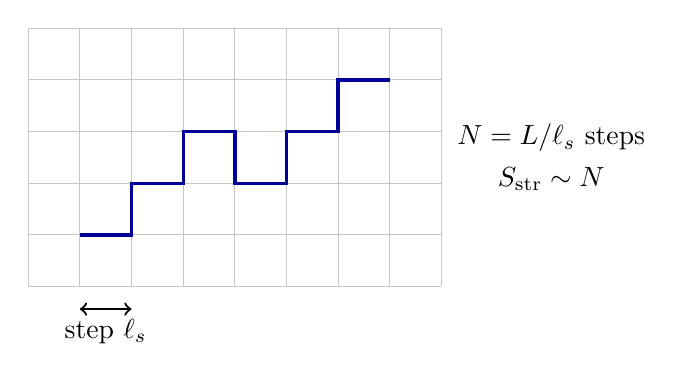
\begin{tikzpicture}[scale=0.82]
  \draw[step=0.8cm,gray!45,thin] (0,0) grid (6.4,4.0);
  \draw[very thick,blue!60!black]
    (0.8,0.8)--(1.6,0.8)--(1.6,1.6)--(2.4,1.6)--(2.4,2.4)--
    (3.2,2.4)--(3.2,1.6)--(4.0,1.6)--(4.0,2.4)--(4.8,2.4)--
    (4.8,3.2)--(5.6,3.2);
  \draw[<->,thick] (0.8,-0.35)--(1.6,-0.35);
  \node[below] at (1.2,-0.35) {step \(\ell_s\)};
  \node[align=center] at (8.1,2.0) {\(N=L/\ell_s\) steps\\[0.3em]\(S_{\mathrm{str}}\sim N\)};
\end{tikzpicture}
\caption{Mô hình mạng trên bảng và cách diễn giải đã được làm gọn của nó theo bước đi ngẫu nhiên. Chính chiều dài đường cong, chứ không phải đường kính của búi rối, quyết định số lựa chọn.}
\lectureframe{00:17:20.000}
\end{figure}

Khối lượng được đếm từ chính các đoạn sơ cấp ấy. Một đoạn có độ dài \(\ell_s\) có thang khối lượng
\begin{equation}
m_{\mathrm{seg}}\sim\frac{1}{\ell_s}.
\end{equation}

\begin{classroomqa}
\audiencequestion{Đoạn sơ cấp có đang được gán độ dài \(\ell_s\) không?\lecturetimestamp{00:18:56}}
\lecturerresponse{Có. Độ dài đặc trưng của nó là \(\ell_s\), nên trong đơn vị tự nhiên khối lượng đặc trưng của nó là \(1/\ell_s\).}
\end{classroomqa}

Cộng \(L/\ell_s\) khối lượng đoạn lại cho ta
\begin{equation}
M\sim\frac{L}{\ell_s}\frac{1}{\ell_s}
=\frac{L}{\ell_s^2},
\qquad
L\sim M\ell_s^2.
\label{eq:l07-string-mass}
\end{equation}
Động năng và thế năng của dây dao động đã được nén vào hệ thức tỉ lệ này; một cách xử lý cơ học thống kê chi tiết cũng cho cùng sự phụ thuộc. Thế vào Phương trình~\eqref{eq:l07-string-entropy-length} ta thu được công thức phía dây mà ta sẽ cần:
\begin{equation}
S_{\mathrm{str}}\sim M\ell_s.
\label{eq:l07-string-entropy-mass}
\end{equation}

\begin{figure}[htbp]
\centering
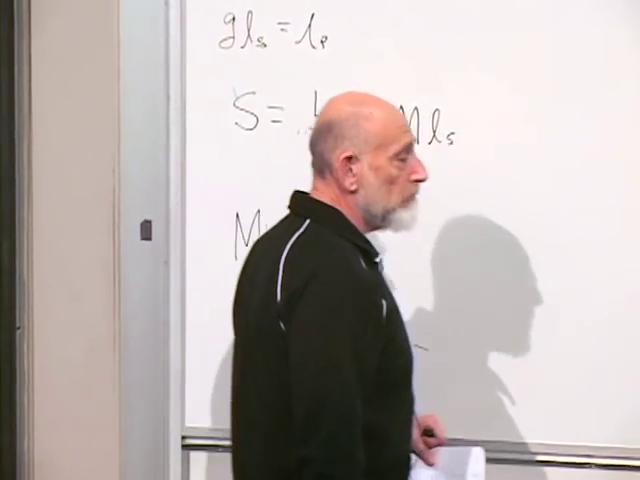
\includegraphics[width=0.66\textwidth]{lecture_07_figure_04.png}
\caption{Cột phía dây được tập hợp trước khi so sánh: \(\ell_p\sim g_s\ell_s\), \(S_{\mathrm{str}}\sim L/\ell_s\sim M\ell_s\) và \(M\sim L/\ell_s^2\).}
\lectureframe{00:21:57.800}
\end{figure}

\section{Vì sao một dây tự do vẫn chưa phải là một lỗ đen}

Ở phía hấp dẫn, công thức bán cổ điển chính xác là
\begin{equation}
S_{\mathrm{BH}}=\frac{A}{4G_N}.
\label{eq:l07-bh-exact}
\end{equation}

\begin{classroomqa}
\audiencequestion{Hệ số số nào nằm ở mẫu số?\lecturetimestamp{00:23:28}}
\lecturerresponse{Là 4. Lập luận tương ứng sẽ khôi phục quy luật tỉ lệ nhưng quá thô để xác định đúng hệ số chính xác đó.}
\end{classroomqa}

Đối với một lỗ đen Schwarzschild bốn chiều,
\begin{equation}
R_s=2G_NM,
\qquad
A=4\pi R_s^2.
\end{equation}
Bỏ qua các hệ số số như bài giảng vẫn làm,
\begin{align}
S_{\mathrm{BH}}
&\sim\frac{A}{G_N}
\sim\frac{(G_NM)^2}{G_N} \\
&\sim M^2G_N
\sim M^2\ell_p^2.
\label{eq:l07-bh-scaling}
\end{align}

\begin{figure}[htbp]
\centering
\includegraphics[width=0.72\textwidth]{lecture_07_figure_06.png}
\caption{Phép so sánh đã hoàn tất trên bảng: entropy dây là một độ dài tính theo đơn vị dây, còn entropy lỗ đen là một diện tích tính theo đơn vị Planck.}
\lectureframe{00:25:35.000}
\end{figure}

Sự giống nhau giữa Phương trình~\eqref{eq:l07-string-entropy-mass} và \eqref{eq:l07-bh-scaling} là gợi ý đáng chú ý, nhưng chúng không phải cùng một công thức. Sẽ là sai nếu chỉ đơn giản gọi lỗ đen ban đầu là một dây tự do rồi thế vào. Phép đếm dây tự do bỏ qua tương tác hút giữa các phần của dây, chính là tương tác nén dây thành một lỗ đen và hạ thấp tổng năng lượng của nó thông qua năng lượng liên kết âm.

Một ngôi sao khiến sai lầm ấy trở nên quen thuộc. Một chất khí nóng có khối lượng sao đặt trong một cái hộp quá lớn không phải là mô hình của một ngôi sao, ngay cả ở cùng nhiệt độ. Tự hấp dẫn làm thay đổi kích thước cân bằng và quan hệ giữa năng lượng với entropy. Việc lần theo mọi tự tương tác của một dây dài sẽ rất khó, nên ta sẽ tránh làm điều đó.

\begin{classroomqa}
\audiencequestion{Nếu một vòng nhỏ rời khỏi một dây dài, entropy của nó giảm. Vậy trao đổi graviton có làm giảm entropy của hệ hấp dẫn không?\lecturetimestamp{00:28:48}}
\lecturerresponse{Không phải trong quá trình trao đổi cân bằng đang được dùng ở đây. Các kích thích ảo được phát ra và hấp thụ theo cả hai chiều; hình vẽ minh họa đó không phải là sự mất đi theo nghĩa đen của một mảnh dây vĩnh viễn. Mục đích duy nhất hiện tại của nó là thiết lập hai thừa số ghép và do đó là sự phụ thuộc theo \(g_s^2\).}
\end{classroomqa}

\section{Trò chơi tương ứng đoạn nhiệt}

Thay vào đó, hãy bắt đầu ở nơi hấp dẫn có thể bỏ qua. Khi \(g_s\to0\), các dây cắt qua nhau mà không tách hay nhập, và lực hút do tự hấp dẫn biến mất. Tăng \(g_s\) trong khi giữ \(\ell_s\) cố định: hấp dẫn mạnh lên, một dây kích thích mạnh co lại, và rốt cuộc nó trở thành một lỗ đen. Vặn ngược núm điều chỉnh một cách chậm rãi thì lỗ đen phải trở về một trạng thái dây. Nó có thể trở thành một số nhỏ các dây dài, nhưng phép đếm năng lượng cao từ bài giảng trước nói rằng ngành trội chứa một dây dài chứ không phải một chất khí khổng lồ gồm các dây ngắn.

\begin{classroomqa}
\audiencequestion{Điều gì được giữ cố định khi hằng số ghép thay đổi?\lecturetimestamp{00:32:19}}
\lecturerresponse{Độ dài dây \(\ell_s\), và do đó thang khối lượng dây sơ cấp \(1/\ell_s\), được giữ cố định. Núm điều chỉnh làm thay đổi \(g_s\) và vì thế \(G_N\sim g_s^2\ell_s^2\).}
\end{classroomqa}

Sự thay đổi phải chậm, cô lập và thuận nghịch. Dưới những điều kiện đó, entropy là một bất biến đoạn nhiệt:
\begin{equation}
\Delta S=0.
\label{eq:l07-adiabatic}
\end{equation}
Chỉ chậm thôi là chưa đủ nếu xảy ra các chuyển tiếp tiêu tán hoặc không được kiểm soát. Ở đây ``đoạn nhiệt'' có nghĩa là có thể theo dõi liên tục cùng một họ trạng thái.\editorialnote{Đây là nghĩa nhiệt động học thuận nghịch của đoạn nhiệt. Một quá trình bất thuận nghịch có thể là đoạn nhiệt theo nghĩa không có dòng nhiệt mà vẫn tạo ra entropy.}

Gọi lỗ đen đích có khối lượng \(M_0\) và hằng số ghép \(g_{s,0}\). Trước khi dùng công thức diện tích mà ta đang tìm cách giải thích, phân tích thứ nguyên chỉ cho biết rằng entropy của một lỗ đen trung hòa, không quay là một hàm nào đó của tổ hợp không thứ nguyên
\begin{equation}
S_{\mathrm{BH}}=f(M\ell_p)
=f(Mg_s\ell_s).
\label{eq:l07-entropy-function}
\end{equation}
Vì vậy, khi giữ \(\ell_s\) cố định, một quỹ đạo đẳng entropy sẽ giữ
\begin{equation}
Mg_s=M_0g_{s,0}
\label{eq:l07-adiabat}
\end{equation}
không đổi, miễn là đi theo cùng một nhánh trạng thái.

Khi \(g_s\) giảm, năng lượng liên kết âm bị loại bỏ, nên khối lượng \(M\) tăng dọc theo quỹ đạo này. Cấu hình dây nền tảng cũng bớt bị liên kết chặt và lan rộng ra. Tuy nhiên, bán kính Schwarzschild hình thức ứng xử như \(R_s\sim Mg_s^2\ell_s^2\sim g_s\ell_s\) trên đường đoạn nhiệt và vì thế giảm.\editorialnote{Trong phần trình bày bằng lời, từ ``nở ra'' được dùng cho vật thể khi được giải phóng khỏi liên kết hấp dẫn. Không nên hiểu điều đó là bán kính Schwarzschild tăng dọc theo đường đoạn nhiệt suy ra ở trên.}

\begin{classroomqa}
\audiencequestion{Vật thể lớn lên hay co lại khi hấp dẫn yếu đi?\lecturetimestamp{00:36:28}}
\lecturerresponse{Cấu trúc dây của nó được giải phóng và nở ra, trong khi khối lượng của nó tăng vì năng lượng liên kết âm bị loại bỏ. Bán kính do công thức lỗ đen gán cho nó giảm xuống cho đến khi chạm thang dây, tại đó mô tả lỗ đen ấy không còn hữu ích nữa.}
\end{classroomqa}

\section{Hai đường cong và giao điểm của chúng}

Biểu diễn khối lượng theo trục đứng và hằng số ghép dây theo trục ngang. Phương trình~\eqref{eq:l07-adiabat} là một đường hyperbol, \(M\propto g_s^{-1}\).

\begin{classroomqa}
\audiencequestion{Loại đường cong nào có tích \(Mg_s\) không đổi?\lecturetimestamp{00:44:08}}
\lecturerresponse{Một đường hyperbol. Đó là đường đoạn nhiệt đi qua điểm đích \((g_{s,0},M_0)\).}
\end{classroomqa}

Đường cong thứ hai đánh dấu chỗ chuyển tiếp giữa hai mô tả. Một lỗ đen không còn có thể được phân giải như một hình học Schwarzschild thông thường một khi bán kính của nó nhỏ hơn một dao động sơ cấp của dây. Vì vậy ta ước lượng điểm tương ứng bằng
\begin{equation}
R_s\sim\ell_s.
\label{eq:l07-correspondence-radius}
\end{equation}
Dùng \(R_s\sim MG_N\) và Phương trình~\eqref{eq:l07-planck-string}, điều này trở thành
\begin{equation}
Mg_s^2\ell_s^2\sim\ell_s,
\qquad
Mg_s^2\sim\frac{1}{\ell_s}.
\label{eq:l07-transition-curve}
\end{equation}
Do đó, đường cong chuyển tiếp đi xuống theo \(M\propto g_s^{-2}\), dốc hơn đường đoạn nhiệt.

\begin{figure}[htbp]
\centering
\includegraphics[width=0.70\textwidth]{lecture_07_figure_07.png}

\vspace{0.6em}
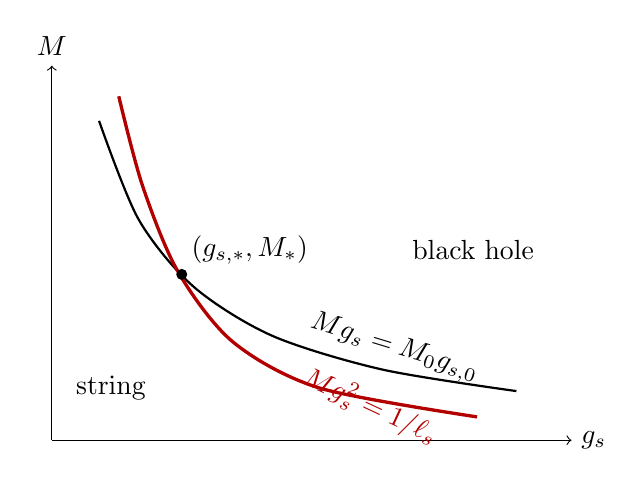
\begin{tikzpicture}[x=1cm,y=0.78cm]
  \draw[->] (0.4,0.4)--(7.0,0.4) node[right] {\(g_s\)};
  \draw[->] (0.4,0.4)--(0.4,6.5) node[above] {\(M\)};
  \draw[thick,black] plot[smooth] coordinates {(1.0,5.6) (1.5,4.0) (2.2,2.9) (3.2,2.1) (4.6,1.55) (6.3,1.2)};
  \draw[very thick,red!70!black] plot[smooth] coordinates {(1.25,6.0) (1.55,4.55) (2.0,3.15) (2.7,2.0) (3.8,1.25) (5.8,0.78)};
  \fill (2.05,3.1) circle (2pt) node[above right] {\((g_{s,*},M_*)\)};
  \node[black,rotate=-17] at (4.75,1.9) {\(Mg_s=M_0g_{s,0}\)};
  \node[red!70!black,rotate=-25] at (4.45,0.95) {\(Mg_s^2=1/\ell_s\)};
  \node at (5.75,3.5) {black hole};
  \node at (1.15,1.25) {string};
\end{tikzpicture}
\caption{Đồ thị trên bảng và cách diễn giải đã được làm gọn của nó. Đường đoạn nhiệt màu đen cắt đường cong tương ứng màu đỏ dốc hơn tại điểm mà vật thể trở nên giống dây.}
\lectureframe{00:49:35.000}
\end{figure}

Tại giao điểm \((M_*,g_{s,*})\), hai phương trình là
\begin{align}
M_*g_{s,*} &= M_0g_{s,0}, \\
M_*g_{s,*}^2 &\sim \frac{1}{\ell_s}.
\end{align}
Bình phương phương trình thứ nhất rồi chia cho phương trình thứ hai:
\begin{equation}
M_*
\sim M_0^2g_{s,0}^2\ell_s.
\end{equation}
Nhân với \(\ell_s\),
\begin{equation}
M_*\ell_s
\sim M_0^2g_{s,0}^2\ell_s^2
\sim M_0^2G_{N,0}.
\label{eq:l07-crossover-result}
\end{equation}

\begin{figure}[htbp]
\centering
\includegraphics[width=0.68\textwidth]{lecture_07_figure_08.png}
\caption{Phần đại số chuyển tiếp đã hoàn tất, bao gồm \(M_*\ell_s=M_0^2g_{s,0}^2\ell_s^2=M_0^2G_{N,0}\).}
\lectureframe{00:54:40.000}
\end{figure}

\begin{classroomqa}
\audiencequestion{Khi chia hai phương trình đường cong cho nhau, \(\ell_s\) phải lên tử hay xuống mẫu?\lecturetimestamp{00:52:41}}
\lecturerresponse{Lên tử. Chia cho \(1/\ell_s\) tức là nhân với \(\ell_s\), nên \(M_*\sim M_0^2g_{s,0}^2\ell_s\).}
\end{classroomqa}

Ở điểm chuyển tiếp, công thức dây là hợp lệ, nên
\begin{equation}
S_*\sim M_*\ell_s.
\end{equation}
Entropy không đổi dọc theo đường đi. Kết hợp mệnh đề này với Phương trình~\eqref{eq:l07-crossover-result} cho entropy của lỗ đen đích ban đầu:
\begin{equation}
S_{\mathrm{BH}}(M_0)
\sim M_0^2G_{N,0}
\sim M_0^2\ell_{p,0}^2.
\label{eq:l07-final-correspondence}
\end{equation}
Đây là dạng tỉ lệ theo định luật diện tích như mong muốn.

\section{Phép tương ứng chứng minh điều gì và không chứng minh điều gì}

Lập luận này không nói rằng lỗ đen ban đầu, với trường hấp dẫn mạnh, là một dây tự do. Nó đưa đối tượng sang một chế độ mà phép đếm dây là đáng tin cậy, đọc entropy ở đó, rồi mang entropy ấy trở lại dọc theo một đường đi thuận nghịch. Sự chuyển tiếp là một crossover chứ không phải một biên pha được xác định sắc nét, nên ước lượng này không thể xác định hệ số \(1/4\) trong Phương trình~\eqref{eq:l07-bh-exact}.

Tuy vậy, cùng logic đó vẫn hoạt động về mặt tham số cho các lỗ đen mang điện, các vật thể đen ở số chiều khác, và các brane đen kéo dài. Các ví dụ đối xứng hơn và siêu đối xứng cho phép các phép đếm trạng thái được bảo vệ, giữ lại thông tin chính xác khi hằng số liên kết thay đổi; các phương pháp ấy khôi phục được các hệ số số học nhưng thêm vào bộ máy toán học không cần thiết cho lập luận khái niệm hiện tại.

Quan trọng nhất, phép tính này cung cấp một diễn giải vi mô. Entropy là bằng chứng của cấu trúc ẩn. Cơ học chất lưu mô tả mật độ, áp suất và dòng chảy trong khi bỏ qua các phân tử; entropy của chất lưu cho thấy rằng những bậc tự do vi mô như vậy quả thực tồn tại. Thuyết tương đối rộng cũng tương tự: nó mô tả một chân trời mà không phô bày các vi trạng thái của nó. Phép đếm dây cho thấy một lý thuyết hấp dẫn lượng tử nhất quán có thể chứa đủ số trạng thái để giải thích entropy của lỗ đen.

\begin{classroomqa}
\audiencequestion{Nếu thay vì kết quả bậc hai mà thu được \(S\sim M^3\ell_p^3\), thì điều đó sẽ có nghĩa gì?\lecturetimestamp{00:59:41}}
\lecturerresponse{Nó sẽ trông như một định luật thể tích. Vật chất thông thường trong một căn phòng hay một tách cà phê có entropy tỉ lệ với thể tích; kết quả bậc hai là đặc biệt vì, thông qua \(R_s\sim M\ell_p^2\), nó tỉ lệ với diện tích chân trời.}
\end{classroomqa}

Kết quả này là bằng chứng rằng entropy Bekenstein--Hawking không chỉ đơn thuần là một phép tương tự nhiệt động học hình thức. Nó chỉ ra các bậc tự do hấp dẫn vi mô, dù phép suy dẫn sơ cấp không làm cho các bậc tự do ấy hiện ra từng cái một.

\section{Từ entropy cực đại đến toàn ảnh}

Bây giờ ta đổi câu hỏi. Thay vì hỏi entropy của một trạng thái xác định, hãy hỏi entropy lớn nhất tương thích với một vùng.

Hãy bắt đầu với một mô hình mạng tinh thể thông thường của một căn phòng. Chia thể tích thành các ô có kích thước \(V_{\mathrm{cell}}\), và cho mỗi ô mang một câu hỏi có-không: bị chiếm hay trống. Susskind đặt cho nguyên tử tưởng tượng cái tên cố ý phi lý ``meatonium'' để không có chi tiết nguyên tử hiện thực nào làm phân tán sự chú ý khỏi phép đếm. Nếu
\begin{equation}
N=\frac{V}{V_{\mathrm{cell}}},
\end{equation}
thì số cấu hình và entropy cực đại là
\begin{equation}
\Omega=2^N,
\qquad
S_{\max}=\log\Omega=N\log2
\sim\frac{V}{V_{\mathrm{cell}}}.
\label{eq:l07-volume-count}
\end{equation}

\begin{figure}[htbp]
\centering
\includegraphics[width=0.68\textwidth]{lecture_07_figure_09.png}
\caption{Căn phòng được chia thành các ô, với hai trạng thái cho mỗi ô. Đây là phép đếm một entropy cực đại, không phải entropy của căn phòng ngăn nắp đang được lớp học chiếm giữ.}
\lectureframe{01:05:20.000}
\end{figure}

Căn phòng thực tế thấp hơn rất xa mức cực đại này. Một trạng thái khảo sát hỗn loạn tất cả những lựa chọn ô đó sẽ cực kỳ nóng. Điều còn lại từ mô hình đồ chơi là kỳ vọng thông thường rằng số bậc tự do độc lập, và do đó entropy cực đại, tỉ lệ với thể tích.

Hấp dẫn lật ngược kỳ vọng đó. Hãy xét một vùng hình cầu có diện tích biên \(A\), entropy ban đầu \(S_{\mathrm{i}}\), và khối lượng \(M\) nhỏ hơn khối lượng \(M_{\mathrm{BH}}\) của một lỗ đen vừa khít lấp đầy hình cầu. Nếu \(M\) lớn hơn, chân trời của nó đã kéo dài ra ngoài biên được chọn rồi.

Bây giờ hãy cho đi vào một vỏ có khối lượng \(M_{\mathrm{BH}}-M\). Thành phần của nó là không liên quan; bài giảng cho phép ánh sáng, vật chất thông thường, hay thậm chí cả pho mát Thụy Sĩ. Hãy sắp đặt để nó sụp đổ. Trạng thái cuối là một lỗ đen có chân trời vừa khít lấp đầy vùng, với entropy
\begin{equation}
S_{\mathrm{f}}=\frac{A}{4G_N}.
\end{equation}
Định luật thứ hai đòi hỏi
\begin{equation}
S_{\mathrm{i}}\le S_{\mathrm{f}}
=\frac{A}{4G_N}.
\label{eq:l07-holographic-bound}
\end{equation}

\begin{figure}[htbp]
\centering
\includegraphics[width=0.70\textwidth]{lecture_07_figure_10.png}

\vspace{0.5em}
\begin{tikzpicture}[scale=0.88]
  \draw[thick] (0,0) circle (1.35);
  \draw[very thick,red!70!black] (0,0) circle (2.05);
  \fill[gray!25] (0,0) circle (1.32);
  \node at (0,0) {\(M,S_{\mathrm{i}}\)};
  \draw[-{Latex[length=3mm]},thick,red!70!black] (3.5,0)--(2.15,0);
  \node[align=center,right] at (3.5,0) {incoming shell\\\(M_{\mathrm{BH}}-M\)};
  \node[below] at (0,-2.2) {final horizon area \(A\)};
\end{tikzpicture}
\caption{Cấu dựng bằng vỏ. Một lượng khối lượng bổ sung vừa đủ được đưa vào trong để hình thành một lỗ đen có chân trời vừa khít lấp đầy vùng đã chọn.}
\lectureframe{01:13:30.000}
\end{figure}

Vì một lỗ đen cỡ đó là một trạng thái được phép và làm bão hòa bất đẳng thức, entropy cực đại là
\begin{equation}
S_{\max}=\frac{A}{4G_N}.
\label{eq:l07-holographic-maximum}
\end{equation}
Đây là nguyên lý toàn ảnh dưới dạng đếm của nó: số tối đa các bậc tự do độc lập trong một vùng có hấp dẫn tỉ lệ với diện tích biên của vùng đó, xấp xỉ một bậc tự do cỡ đơn vị trên mỗi diện tích Planck, thay vì tỉ lệ với số thể tích Planck ở bên trong.\editorialnote{Lập luận vỏ giả sử rằng vùng có thể được bao kín và làm sụp đổ theo cách đã nêu. Các không-thời gian tổng quát hơn đòi hỏi các cận entropy hiệp biến, nhưng lập luận hình cầu nắm bắt đúng nguyên lý được dùng trong bài giảng.}

Sự chênh lệch là khổng lồ. Trực giác lý thuyết trường địa phương gợi rằng những lựa chọn được thực hiện tại các điểm bên trong khác nhau phải kết hợp độc lập, tạo ra một định luật thể tích. Hấp dẫn nói rằng đủ nhiều lựa chọn như vậy tự chúng sẽ sụp đổ, và lỗ đen cung cấp entropy cho phép lớn hơn. Vì thế phép đếm trên biên không phải là một hiệu chỉnh nhỏ đối với phép đếm theo thể tích; nó là một cách tổ chức khác của không gian Hilbert.

\begin{classroomqa}
\audiencequestion{Điều gì xảy ra đối với một vũ trụ rất lớn có mật độ gần như đồng đều?\lecturetimestamp{01:15:48}}
\lecturerresponse{Câu hỏi đó đòi hỏi vũ trụ học chứ không phải cấu dựng hình cầu tĩnh. Nó thúc đẩy sự chuyển ngay sang các nghiệm giãn nở của phương trình Einstein.}
\end{classroomqa}

\begin{classroomqa}
\audiencequestion{Cận diện tích có liên quan đến nguyên lý bất định không?\lecturetimestamp{01:16:03}}
\lecturerresponse{Bài giảng để ngỏ câu hỏi này và tiếp theo chuyển sang vũ trụ học.}
\end{classroomqa}

\section{Không gian giãn nở}

Ở đây chúng ta sẽ không suy ra các nghiệm vũ trụ học từ các phương trình Einstein; chúng ta sẽ viết các nghiệm đó ra và học cách đọc chúng. Các lát cắt không gian có thể cong dương và kín, cong âm và hyperbolic, hoặc phẳng. Trong thảo luận hiện tại, hãy lấy các lát cắt Euclid phẳng theo không gian trong một không-thời gian phụ thuộc thời gian.

\begin{classroomqa}
\audiencequestion{Tương tự không-thời gian của không gian Euclid thông thường là gì?\lecturetimestamp{01:19:37}}
\lecturerresponse{Không-thời gian Minkowski. Mô hình vũ trụ học được xét ở đây có các lát cắt không gian phẳng nhưng không phải là không-thời gian Minkowski, vì metric không gian của nó thay đổi theo thời gian.}
\end{classroomqa}

Hình ảnh quả bóng bay quen thuộc mô tả một bề mặt kín đang giãn nở thấp hơn một chiều. Susskind nhắc lại việc đã thử làm minh họa đó với một quả bóng lớn có đánh dấu; bút đánh dấu làm cao su yếu đi và gây ra một tiếng nổ theo nghĩa đen. Sự cố ấy cũng bộc lộ một khuyết điểm khái niệm của phép loại suy. Khi một quả bóng thông thường nở ra, các phân tử cao su của nó tách xa nhau và vật liệu mỏng dần cho đến khi vỡ. Không gian vũ trụ học không có các định luật địa phương bị pha loãng. Để bảo toàn phép loại suy, ta phải hình dung rằng các phân tử cao su mới liên tục được chèn thêm vào sao cho mỗi mảng nhỏ đều giữ nguyên các tính chất địa phương như cũ. Trong một mô hình phẳng, hãy thay quả bóng bằng một tấm lớn được kéo đều ra ngoài và cũng được bổ sung tương tự.

Về mặt toán học, sự giãn nở nằm trong metric:
\begin{equation}
\begin{aligned}
ds^2&=-dt^2+a(t)^2d\mathbf{x}^2,\\
d\mathbf{x}^2&=\delta_{ij}\,dx^i dx^j
=dx^2+dy^2+dz^2.
\end{aligned}
\label{eq:l07-frw-metric}
\end{equation}

\begin{figure}[htbp]
\centering
\includegraphics[width=0.72\textwidth]{lecture_07_figure_11.png}
\caption{Metric giãn nở với lát cắt không gian phẳng như được viết trên bảng.}
\lectureframe{01:25:10.000}
\end{figure}

Những điểm giữ cố định các tọa độ không gian được gọi là đồng chuyển động. Nếu hai điểm như vậy có độ tách tọa độ \(\Delta x\), thì khoảng cách riêng của chúng tại thời điểm \(t\) là
\begin{equation}
D(t)=a(t)\Delta x.
\label{eq:l07-proper-distance}
\end{equation}
Tọa độ của chúng không chuyển động, nhưng khoảng cách metric giữa chúng thay đổi. Lấy đạo hàm tại \(\Delta x\) cố định,
\begin{equation}
V=\dot D=\dot a\,\Delta x
=\frac{\dot a}{a}D.
\end{equation}
Định nghĩa tham số Hubble
\begin{equation}
H(t)=\frac{\dot a(t)}{a(t)}.
\label{eq:l07-hubble-parameter}
\end{equation}
Khi đó
\begin{equation}
V=H(t)D,
\label{eq:l07-hubble-law}
\end{equation}
đó là định luật Hubble tại một thời điểm vũ trụ cố định.

\begin{figure}[htbp]
\centering
\includegraphics[width=0.68\textwidth]{lecture_07_figure_12.png}
\caption{Định luật lùi xa tại cùng thời gian trên bảng: \(V=D\,\dot a/a\).}
\lectureframe{01:29:10.000}
\end{figure}

Tên gọi ``hằng số Hubble'' có thể gây hiểu lầm. Nói chung, \(H(t)\) thay đổi theo thời gian. Đại lượng không đổi theo không gian là tỉ số \(V/D\) đối với mọi cặp điểm đồng chuyển động trên cùng một lát thời gian.

\begin{classroomqa}
\audiencequestion{Đối với các thiên hà xa, thời gian nào xuất hiện trong hệ thức này? Ta quan sát chúng ở một thời kỳ sớm hơn.\lecturetimestamp{01:31:10}}
\lecturerresponse{Phương trình~\eqref{eq:l07-hubble-law} là một mệnh đề tại cùng thời gian. Một quan sát đi theo một tia sáng hướng về quá khứ và lấy mẫu thiên hà xa ở một thời điểm sớm hơn, nên quan hệ giữa độ dịch đỏ đo được và khoảng cách đòi hỏi toàn bộ lịch sử trên nón ánh sáng chứ không phải một giá trị tức thời duy nhất của \(H\).}
\end{classroomqa}

\begin{figure}[htbp]
\centering
\includegraphics[width=0.66\textwidth]{lecture_07_figure_13.png}
\caption{Bản phác thảo không-thời gian dùng để phân biệt một độ tách tại cùng thời gian với điều mà người quan sát thấy dọc theo một tia sáng hướng về quá khứ.}
\lectureframe{01:33:20.000}
\end{figure}

\section{Thang Hubble và sự giãn nở de Sitter}

Trong đơn vị \(c=1\), Phương trình~\eqref{eq:l07-hubble-law} gán tốc độ lùi xa bằng 1 tại khoảng cách
\begin{equation}
D_H=\frac{1}{H}.
\label{eq:l07-hubble-radius}
\end{equation}
Các điểm đồng chuyển động xa hơn có thể có \(V>1\), thậm chí \(V\gg1\), mà không vi phạm thuyết tương đối hẹp. Chúng không đi ngang qua một người quan sát địa phương nhanh hơn ánh sáng; khoảng cách riêng giữa chúng tăng lên vì hình học ở giữa đang giãn nở.\editorialnote{Đối với một vũ trụ học tổng quát phụ thuộc thời gian, \(1/H\) là bán kính Hubble, không tự động là một chân trời sự kiện. Nó trở thành thang chân trời không đổi trong trường hợp de Sitter sẽ được bàn tiếp theo.}

Trong nhiều mô hình vũ trụ học cũ hơn, chậm dần, \(H(t)\) giảm và \(1/H(t)\) tăng, nên những vùng từng lùi xa siêu quang về sau có thể đi vào liên hệ nhân quả. Trái lại, bức tranh thời muộn được bàn trong bài giảng tiến tới một hằng số dương \(H\). Khi đó \(1/H\) giữ nguyên, và phương trình giãn nở trở thành
\begin{equation}
\frac{\dot a}{a}=H,
\qquad
\dot a=Ha.
\label{eq:l07-constant-h}
\end{equation}

\begin{classroomqa}
\audiencequestion{Đơn vị của một tham số Hubble không đổi là gì?\lecturetimestamp{01:38:24}}
\lecturerresponse{Nghịch đảo thời gian. Tương đương, với \(c=1\), nó là nghịch đảo độ dài. Đại lượng \(H^{-1}\) cung cấp cả một thang thời gian giãn nở lẫn một thang khoảng cách; bài giảng dùng một ví dụ bậc độ lớn cỡ mười lăm tỷ năm.}
\end{classroomqa}

Nghiệm của Phương trình~\eqref{eq:l07-constant-h} là
\begin{equation}
a(t)=a_0e^{Ht}.
\label{eq:l07-desitter-scale-factor}
\end{equation}

\begin{classroomqa}
\audiencequestion{Hàm nào có tốc độ biến thiên tỉ lệ với chính nó?\lecturetimestamp{01:39:04}}
\lecturerresponse{Một hàm mũ. Vì vậy thừa số tỉ lệ là \(a_0e^{Ht}\), còn hệ số không gian \(a(t)^2\) trong metric tăng như \(e^{2Ht}\).}
\end{classroomqa}

\begin{figure}[htbp]
\centering
\includegraphics[width=0.70\textwidth]{lecture_07_figure_14.png}
\caption{Các phương trình với \(H\) không đổi và nghiệm hàm mũ của chúng trên bảng.}
\lectureframe{01:39:30.000}
\end{figure}

Một không-thời gian có sự giãn nở hàm mũ này là không gian de Sitter. Thang Hubble không đổi của nó tạo ra một chân trời sự kiện ở khoảng cách riêng hữu hạn. Theo một nghĩa nào đó, hình học này là phần bù của bức tranh lỗ đen: một người quan sát ở bên trong một chân trời vũ trụ học, còn các vật thể đủ xa thì lùi ra xa và không bao giờ có thể gửi các tín hiệu bắt kịp người quan sát. Chân trời lỗ đen che giấu miền bên trong khỏi một người quan sát bên ngoài; chân trời de Sitter che giấu miền bên ngoài của mảng không-thời gian mà người quan sát có thể tiếp cận. Không giống một lỗ đen thông thường đang bay hơi, hình học de Sitter lý tưởng ở đây được xem là tồn tại bền vững. Sự so sánh mới chỉ bắt đầu ở đây. Bài giảng tiếp theo sẽ phát triển chân trời này, nhiệt động học của nó và những câu đố mà nó tạo ra cho vũ trụ học.